\documentclass[10pt,a4paper]{article}

\usepackage{amsmath}
\usepackage{amssymb}
\usepackage{graphicx}
\usepackage{float}
\usepackage[polish]{babel}
\usepackage[utf8]{inputenc}
\usepackage{polski}
\usepackage{listings}
\frenchspacing
\lstset{basicstyle=\ttfamily,
  showstringspaces=false,
  breaklines=true,
  numbers=left,
  captionpos=b,
  language=bash,
  frame=single
}

\author{Marcin Ochman}
\title{Programowanie liniowe - algorytm SIMPLEX}

\begin{document}
\maketitle

\section{Opis problemu}

Na samym początku, chciałbym przybliżyć teoretyczne podejście do problemów 
optymalizacyjnych.

\subsection{Problem optymalizacyjny}
Często mamy do czynienia z problemami optymalizacyjnymi tzn. szukamy pewnych argumentów
$x_0,x_1,x_2,x_3...$ takich, aby funkcja $f(x_0,x_1,x_2,x_3,...)$
przyjmowała minimalną lub maksymalną wartość tj.
\begin{equation}
x_0,x_1,x_2,x_3...\xrightarrow{}min\{f(x_0,x_1,x_2,x_3) \}
\end{equation}
\begin{equation}
x_0,x_1,x_2,x_3...\xrightarrow{}max\{f(x_0,x_1,x_2,x_3) \}
\end{equation}
Zdarza się jednak, że mamy do czynienia z góry określonymi ograniczeniami:
\begin{equation}
\label{ograniczenia}
\begin{aligned}
g_1(x_0,x_1,x_2,x_3,...)&\le c_1\\
g_2(x_0,x_1,x_2,x_3,...)&\le c_2\\
&...
\end{aligned}
\end{equation}
wtedy, musimy szukać optymalnego rozwiązania w zbiorze określonym przez nierówności \ref{ograniczenia}. 
Liniowość problemu upraszcza go tak, że nasze funkcje $f,g_1,g_2,...$ wyglądają następująco:

\begin{equation}
\begin{aligned}
f(x_0,x_1,x_2,x_3,...)=c_0x_0+c_1x_1+c_2x_2+c_3x_3,...\\
a_{0,0}x_0+a_{0,1}x_1+a_{0,2}x_2+a_{0,3}x_3,...&\le b_1\\
a_{1,0}x_0+a_{1,1}x_1+a_{1,2}x_2+a_{1,3}x_3,...&\le b_2\\
&... 
\end{aligned}
\end{equation}
Przy czym:
\begin{equation*}
c_0,c_1..., a_{0,0},a_{0,1}...,a_{1,0},a_{1,1}... \in \mathbb{R}
\end{equation*}
Jednym z algorytmów, który potrafi znaleźć optymalne rozwiązanie takiego problemu, jest
SIMPLEX, który omówię w następnym podrozdziale.

\subsection{Krótki opis algorytmu SIMPLEX}
Jest to jeden z najczęściej stosowanych algorytmów optymalizacyjnych. Swoją popularność 
zawdzięcza przede wszystkim swojej prostocie. Nazwa tego algorytmu wzięła się od sympleksu, czyli
trójkąta uogólnionego na więcej wymiarów. Algorytm pracuje na pewnym zbiorze rozwiązań
dopuszczalnych wynikających z przyjętych ograniczeń np.dla dwóch zmiennych mamy ograniczony 
powierzchnię, dla trzech zmiennych mamy ograniczoną przestrzeń itd. Z każdym krokiem
iteracyjnym wyznaczany jest nowy wierzchołek, jeśli poprawia on wcześniejsze rozwiązanie, pętla
jest kontynuowana, jeśli nie algorytm kończy swoje działanie. Kolejne wierzchołki są wyznaczane
na podstawie tablicy sympleksowej. Dla problemu poruszonego w dalszej części sprawozdania, na 
samym początku tablica wygląda następująco:

\begin{table}[ht]
\centering
\begin{tabular}{|c|c|c|c|c|c|c|c|}
\hline
 ---& $x_0$ & $x_1$ & $s_0$ & $s_1$ & $s_2$ & $p$ & b\\
\hline
$s_0$ & 1 & 0 & 1 & 0 & 0 & 0 & 4\\
\hline
$s_1$ & 0 & 2 & 0 & 1 & 0 & 0 & 12\\
\hline 
$s_2$ & 3 & 2 & 0 & 0 & 1 & 0 & 18\\
\hline
$p$ & -3000 & -5000 & 0 & 0 & 0 & 1 & 0\\
\hline
\end{tabular}
\caption{Tablica sympleksowa na samym początku działania algorytmu}
\end{table}

Zasada tworzenia takiej tablicy jest dosyć prosta. Każde ograniczenia zamieniamy na równanie, 
dodając kolejną zmienną ze współczynnikiem 1. W naszym przypadku mamy 3 dodatkowe zmienne 
$s_0,s_1,s_2$ - tyle ile jest ograniczeń. Następnie wpisujemy równania do tabeli. Warto wspomnieć
o pierwszej kolumnie, na samym początku wpisujemy tam zmienne dodatkowe. Mamy również tam zmienną
$p$, która w ogólności wyraża się wzorem: 
\begin{equation*}
p+f(x_0,x_1,...)=0
\end{equation*}
stąd mamy ujemne współczynniki przy 3000 i 5000. W każdym kroku algorytmu wykonujemy odpowiednie 
operacje:
\begin{itemize}
\item wybieramy kolumnę piwotu - najmniejszy element w wierszu $p$
\item wybieramy wiersz, w którym iloraz elementu z kolumny b i z kolumny piwotu jest najmniejszy
\item aktualizujemy pierwszą kolumnę zmiennych - wpisujemy do wybranego wiersza w pierwszej 
kolumnie odpowiednią zmienną z pierwszego wiersza i kolumny piwotu
\item mnożymy wybrany wiersz tak, aby piwot był równy 1
\item dodajemy lub odejmujemy tyle razy wiersz do pozostałych wierszy tak, aby elementy na górze 
i na dole piwotu stały się zerami
\end{itemize}

W ten sposób powtarzamy powyższe kroki, aż do momentu, kiedy nie będzie ujemnych wartości
w ostatnim wierszu. Na samym końcu należy zinterpretować wynik:
\begin{itemize}
\item w pierwszej kolumnie mamy jakiej zmiennej odpowiada wartość z ostatniej kolumny - ta 
wartość to znalezione rozwiązanie
\item w komórce w ostatnim wierszu ostatniej kolumny mamy wartość funkcji, jaką ona przyjmuje
dla znalezionych argumentów
\end{itemize}
\begin{table}[ht]
\centering
\begin{tabular}{|c|c|c|c|c|c|c|c|}
\hline
 ---& $x_0$ & $x_1$ & $s_0$ & $s_1$ & $s_2$ & $p$ & b\\
\hline
$x_0$ & 0 & 0 & 1 & $\frac{1}{3}$ & -$\frac{1}{3}$ & 0 & 2\\
\hline
$x_1$ & 0 & 1 & 0 & 0.5 & 0 & 0 & 6\\
\hline 
$x_0$ & 0 & 0 & 1 & $\frac{1}{3}$ & -$\frac{1}{3}$ & 0 & 2\\
\hline
$p$ & 0 & 0 & 0 & 1500 & 1000 & 1 & 36000\\
\hline
\end{tabular}
\caption{Tablica sympleksowa przy zakończeniu działania algorytmu}
\end{table}

\section{Zadanie optymalizacyjne do rozwiązania}
Moim zadaniem było napisanie programu, który rozwiąże zadanie optymalizacyjne za pomocą 
algorytmu SIMPLEX, którego treść została przedstawiona poniżej.

\subsection{Treść zadania}
Znaleźć, dla jakiego $x_0,x_1$ funkcja $f(x_0,x_1)=3000x_0+5000x_1$ przyjmie wartość 
maksymalną, przy podanych ograniczeniach:
\begin{equation}
\begin{aligned}
x_0&\le 4\\
x_1&\le 12\\
3x_0+2x_2&\le 18\\
x_0&\le 0\\
x_1&\le 0
\end{aligned}
\end{equation}

\subsection{Rozwiązanie zadania ,,na kartce''}

Narysujmy najpierw przestrzeń dozwolonych rozwiązań. 
\begin{figure}[H]
\centering
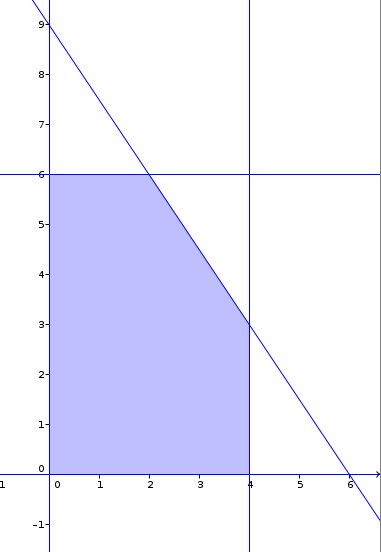
\includegraphics[width=0.3\linewidth]{./Wykresy/obszar}
\caption{Zbiór rozwiązań dopuszczalnych}
\label{fig:obszar}
\end{figure}

Następnie wyznaczmy wierzchołki tego wielokąta, ponieważ dla wierzchołków funkcja
będzie przyjmowała wartości ekstremalne:

\begin{table}[ht]
\centering
\begin{tabular}{|c|c|c|}
\hline
$x_0$ & $x_1$ & $f(x_0,x_1)$ \\
\hline
0 & 0 & 0 \\
\hline
4 & 0 & 12000 \\
\hline
4 & 3 & 27000 \\
\hline
2 & 6 & 36000 \\
\hline
0 & 6 & 30000 \\
\hline
\end{tabular}
\end{table}

Jak widać, dla punktu $(2,6)$ funkcja $f(x_0,x_1)$ przyjmuje wartość maksymalną - jest to 
poszukiwane rozwiązanie naszego problemu, aby to potwierdzić na Rysunku \ref{fig:wykres} został 
przedstawiony wykres poziomicowy funkcji celu.

\begin{figure}
\centering
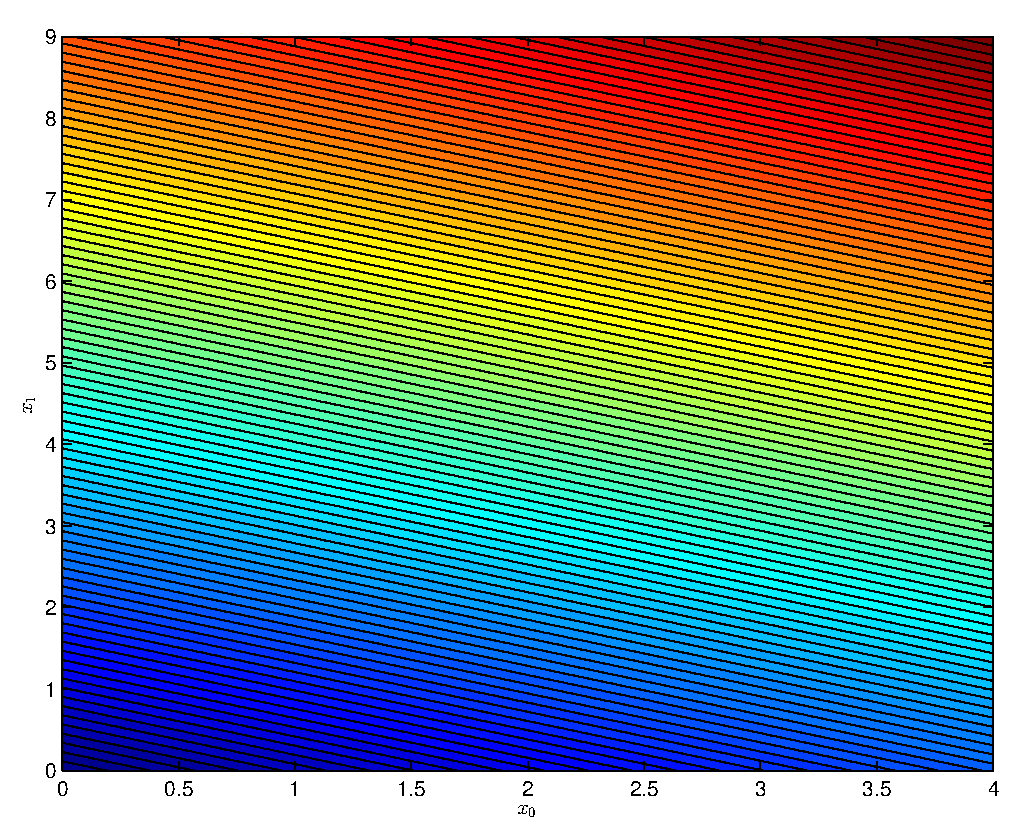
\includegraphics[width=0.7\linewidth]{./Wykresy/wykres}
\caption{Wykres funkcji celu}
\label{fig:wykres}
\end{figure}


\subsection{Rozwiązanie zadania przez komputer}

Poprawny wynik tego zadania, rozwiązany przez program znajduje się poniżej. Jest on
oznaczony jako Problem nr 1.

\begin{lstlisting}[caption={Wyjście konsoli, pokazujące, działanie napisanego programu.}]
******************************
PROBLEM nr 1:

Maksymalizacja: f(x0, x1)=3000*x0+5000*x1
Przy ograniczeniach:
1*x0+0*x1<=4
0*x0+2*x1<=12
3*x0+2*x1<=18

Rozwiazanie: (2, 6)
Wartosc funkcji: 36000

******************************
PROBLEM nr 2:

Maksymalizacja: f(x0, x1, x2)=7*x0+8*x1+10*x2
Przy ograniczeniach:
2*x0+3*x1+2*x2<=1000
1*x0+1*x1+2*x2<=800

Rozwiazanie: (200, 0, 300)
Wartosc funkcji: 4400

******************************
\end{lstlisting}


\section{Wnioski oraz uwagi}
Na podstawie przeprowadzonego ćwiczenia, można dojść do następujących wniosków:
\begin{itemize}
\item Algorytm SIMPLEX, zarówno dla Problemu nr 1 jak i dla Problemu nr 2 wyznaczył
optymalne rozwiązanie
	\item Implementacja algorytmu była bardzo prosta i szybka
	\item Jest bardzo dużo rzeczywistych problemów optymalizacyjnych, które mogą być
		rozwiązywane za pomocą algorytmu SIMPLEX m.in
	\begin{itemize}
		\item minimalne koszty produkcji
		\item maksymalny zysk firmy
		\item wybór odpowiedniej drogi przy transporcie
		\item i wiele innych
	\end{itemize}
\end{itemize}
\end{document}